\chapter{Users who can benefit from the project}\label{ch:End-User} 
There is two main types of amputees, persons who is born without a limb, and persons whom lost a limb due to trauma or a diseases, like diabetes\cite{StrainInjuries}. There many types of amputees under the main types, some are missing a toe where others have lost an arm or leg, this project will focus on a person with a very high level amputation specifically shoulder disarticulation.\\

\section{Shoulder disarticulation}
An amputee with shoulder disarticulation have their arm amputated at the shoulder. A generalised description of different arm amputations situation is, see figure \ref{fig:Degrees_of_amputations}:

\begin{figure}[H]
    \centering
    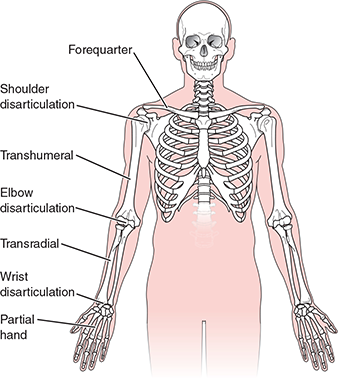
\includegraphics[width=8cm,height=7cm]{Figures/Contextual_figures/Degrees_of_amputation.png}
    \caption{Degrees of amputations, including shoulder disarticulation}
    \label{fig:Degrees_of_amputations}
\end{figure}
Here the arm is separated with the humerus but the shoulder-socket remains. This leaves some mussel and mobility of the shoulder-joint itself intact.  
%%%%%%%%%%%%%%%%%%%%%%%%%%%%%% Lad os se om det virker uden %%%%%%%%%%%%%%%
%\paragraph{Health care}
%In Denmark the Health care system will help the citizen acquire a needed prosthesis and the medical help needed in this process.
%However this is within reason, an example is in Ringkøbing-Skejren municipality, the average spending on each of their 44 user is 35000 DKK\cite{rksk}. A higher levelled prostheses will normally not be provided by the municipality.

%\paragraph{Pre-amputees}
%The degree of amputation is determined in a consultation between the individual and a doctor. This will allow the person whom has to undergo the surgery to be a part of the decision, at time even deciding if it is better to have a amputation above or below a certain point \cite{rksk}. As a result the type of prosthesis and control system is determined.\\
%%%%%%%%%%%%%%%%%%%%%%%%%%%%%%%%%%%%%%%%%%%%%%%%%%%%%%%%%%%%%%%%%%%%%%%%%%%

\section{Difficulties} \label{Difficoulties}
Severe amputees and loss of limbs creates obstacles on a daily basis.Here a prostheses can be a tremendous help, in order to live a life, where the user still can function independently and do daily tasks.  Some of the difficulties for upper limb amputees who uses prostheses is listed bellow.\\

\subsection*{Skin care}
The residual limb is enclosed in the prosthesis which is sealed airtight around the limb. This leads to sweat not being able to evaporate.\\
Exposing the limb to such components will result in blisters and irritated skin around the residual limb\cite{SkinCare}.\\

\subsection*{Repetitive Strain Injuries}\\
Physical overloads caused by the joint of the prosthetic fitting with pain as a result is another well-known issue. Vibrations, rotations and mechanical pressures can amplify the pain.\\
According to research from an Australian survey (1999)  show that amputees is more likely to get an repetitive strain injury, in fact  the research show that half of the people with prosthesis tested feels pain while operating repetitive tasks, while non-amputees reports that, only 10 percent feels the pain \cite{StrainInjuries}.\\

\subsection*{Weight Control}\\
The users weight can fluctuate, resulting in different sizes on the attachment of the prostheses. If weight is gained, the size of the attachment might get too small, resulting in an imperfect fit causing pain.\\
This project will not make a fluctuating attachment and see it as the users duty to conserve the weight and height the amputee had, when the prosthesis was attached\cite{weightControl}.

\section{Conclusion}
The end user of the project is a person with a high level of amputation. Living without a limb creates a lot of difficulties for the individual to overcome.\\
In the next chapter the project looks into which options are available to ease these difficulties and some part-solutions on which systems could be looked at when controlling e.g a prostheses. 